\chapter{Methodology}

In this section, the methodology of the proposed solution is explained in detail. This section is divided into sequential subsections that each descibe a step in the process used to arrive at the proposed dataset, the formulation of the analytical problem to be solved, and the \acrfull{ml} related data preparation, training, and evaluation.

\section{General approach overview}

Based on the findings from the literature review conducted in \cref{sec:lit_review}, it is clear that the existing work is limited in terms of a general and global prediction solution for vessel destination ports. Thus, this thesis proposes a method that is able to predict vessels' future destination ports using a combination of positional data from the \gls{aivdm} protocol and vessel segmentation values. This is an important objective of the thesis as no related studies seem to take additional vessel information into account. The proposed solution is not restricted by specific geographical regions nor time intervals and should form a foundation of which it is possible to extend with more features, or data attributes, regarding the traveling vessels and voyages. The method of developing the proposed solution can be divided into the following steps:

\begin{enumerate}
    \item Construct voyages and trajectories using a voyage definition derived from the departure and arrival detection described in \cref{sec:vessel_transitions}.
    \item Sample, or simplify, the trajectories to make them more comparable using vessel similarity measurement methods.
    \item Calculate the \acrfull{mstd} and the similarity value for every voyage's trajectory.
    \item Collect the historical data attributes to be used for \acrfull{ml} including departure and arrival ports, vessel segmentation values, \acrshort{mstd} values, and trajectory lengths.
    \item Train a \acrshort{ml} model to predict the arrival ports of voyages using the dataset constructed.
\end{enumerate}

\section{The initial data processing}

This section describes the initial dataset used in the proposed solution which is later processed and used to train a \acrshort{ml} model for predictions. This data foundation is provided to the author by \acrfull{mo}. Moreover, for this thesis, data used in the analysis is stored in a separate, dedicated PostGreSQL database also hosted in \acrshort{mo}'s cloud computing environment.

\subsection{Positional historical AIS data}

The first step in the dataset processing is to collect a historical set of \acrshort{ais} data. In this thesis, this data provided by \acrshort{mo} contains more than 1.5 billion positional records for over 65 000 unique vessels starting from December 2019 and is continuously collected. In this thesis, circa 1.2 billion records ranging from December 2019 to March 2021 was used for the proposed solution. The historical records were copied in batches from \acrshort{mo}'s database into a separate database used in this thesis in a table called \textit{vessel positions history}. This table contains the following relevant attributes for each historical record:

\begin{itemize}
    \item id - a sequential identifier
    \item imo - the \acrshort{imo} number of the vessel that transmitted the position.
    \item mmsi - the \acrshort{mmsi} number of the vessel that transmitted the position.
    \item position - a geographical coordinate of the vessel in the \textit{Mercator} projection.
    \item timestamp - the unix timestamp (seconds since Unix Epoch) of when the position was transmitted by the vessel.
\end{itemize}

In the process of copying data to the dedicated database, each position's coordinate is validated by ensuring that it follows the bounds its projection, i.e., that the longitude value is between -180, and 180 degrees, and the latitude is between -90, and 90 degrees. If a coordinate has invalid values, it is disregarded. Furthermore, positions that lie exactly on the north and south bounds, or exactly at coordinates \textit{(180, 90)} and \textit{(-180, -90)} are also disregarded as these positions are impossible places to navigate but is still frequently seen in the database. \cref{fig:ais_positions} in \cref{sec:ais_data} shows a visualization of an extract of 100 million records from the historical \acrshort{ais} database which shows the extent of the collected positions.

Furthermore, as also mentioned in \cref{sec:ais_data}, \acrshort{imo} numbers and \acrshort{mmsi} numbers are divided up in the positional and static \acrshort{ais} reports. Therefore, \acrshort{mmsi} numbers in positional data must be matched to \acrshort{imo} numbers in the static information (which contains both) to collect both identifiers in the historical \acrshort{ais} database. The \acrshort{imo} identifier is required to extract information such as vessel segments and sub-segments as these are initially constructed using information from static records. Positions transmitted by a \acrshort{mmsi} number that does not map to a known \acrshort{imo} number, or have invalid values for either, are disregarded. The validity of both values can be determined following the \gls{aivdm} protocol which defines how these numbers are constructed and used.

\subsection{Segments}

As described in \cref{sec:vessel_info_segments}, vessel segmentation values are additional attributes that indicate a vessel's type, dimensions, and capacity. These labels are thought to provide insight into traveling patterns of vessels. Thus, this information is important for this thesis' proposed solution. \acrshort{mo} has vessel segmentation information for every unique vessel collected by \acrshort{ais} data. This information is collected and stored in the dedicated database in a table called \textit{vessel segments}. This table contains information per vessel and has the following relevant attributes:

\begin{itemize}
    \item imo - the \acrshort{imo} number of the vessel.
    \item segment - the vessel's segment value, e.g. \textit{dry bulk}, \textit{tanker}, \textit{chemical}, etc\ldots
    \item sub-segment - the vessel's sub-segment value, e.g., \textit{mini bulker}, \textit{handysize}, \textit{panamax}, etc\ldots
\end{itemize}

Finally, it is worth noting that some vessels can function as two different types of vessels such as tanker vessels that also functions as chemical transport vessels. These ``combo'' vessels contains multiple entries in the segmentation database table for each of the function it serves. However, they also contain a dedicated entry where the segment value is ``combo'' which can have a specific range of sub-segments. For analysis, it is more practical to assume that every vessel only has one segment and one sub-segment, therefore, for combo vessels, only the combo segment and sub-segment is considered.

\subsection{Ports}

Next, the traveling vessel's departure and arrival port are required to predict vessels' future destinations, as destinations are defined ports. As already described in \cref{sec:shipping_ports}, \acrshort{mo} has a large number of ports available in a port database out of which around 5600 are considered relevant for the shipping industry. For this thesis, only these 5600 relevant ports are considered for the analysis, thus, these are also stored in the dedicated database in a table called ``ports''. This table contains the following relevant attributes:

\begin{itemize}
    \item locode - the port's unique identifier following the \gls{locode} protocol.
    \item position - the port's geographical coordinates specified in the Mercator projection.
    \item name - a text value for the name of the port.
\end{itemize}

\subsection{Vessel transitions}

As described in \cref{sec:vessel_transitions}, vessel transitions are historical events where a vessel's \acrshort{ais} navigational status transitions from a status indicating that it is moving to the status ``MOORED'' and vice versa. These events are mapped geographically to the closest known port within a 25 kilometer radius, thus, vessel transitions provide a historical record of port arrivals and departures. \acrshort{mo} has more information available in their transition data, however, only vessel arrival and departure data is of relevance to the proposed solution. The relevant data is stored in the dedicated database as a table called \textit{vessel transitions}. This table contains vessel identifiers, the event's mapped port, the Unix timestamp of when the event occurred, and the transition type indicating whether the vessel arrived or departed. \cref{tab:vessel_transitions_example} shows an example extract from the transitions data for a single vessel. It shows that when sorted by time, the events follow a pattern of sequential arrival and departures from different ports.

\begin{table}[htbp]
    \centering
    \begin{tabular}{p{0.7in} p{0.9in} p{1in} p{1in} p{0.65in}}
    \hline
    \bfseries{IMO} & \bfseries{MMSI} & \bfseries{Transition} & \bfseries{Timestamp} & \bfseries{Port Code} \\ \hline
        9824083 & 538008866 & ARRIVAL   & 1595383670 & KRONS \\ \hline
        9824083 & 538008866 & DEPARTURE & 1596177702 & KRONS \\ \hline
        9824083 & 538008866 & ARRIVAL   & 1599869735 & BRITQ \\ \hline
        9824083 & 538008866 & DEPARTURE & 1600002777 & BRITQ \\ \hline
        9824083 & 538008866 & ARRIVAL   & 1603942962 & CNZNG \\ \hline
        9824083 & 538008866 & DEPARTURE & 1604191770 & CNZNG \\ \hline
    \end{tabular}
\caption{Example rows for a single vessel in the vessel transitions table}
\label{tab:vessel_transitions_example}
\end{table}

\section{Vessel voyage definition}

\begin{itemize}
    \item Transitions
    \item (Clustering)
\end{itemize}

\subsection{Transition voyages}

\begin{itemize}
    \item Extracting departure=>arrival times grouped by vessels, ordered by time
    \item Finding position reports between each timestamp for given vessel
    \item Constructing trajectory (3D trajectory with timestamps)
    \item Validating trajectory, noise filtering
\end{itemize}

\section{Data processing for \acrfull{ml}}

\subsection{Trajectory sampling}

\begin{itemize}
    \item Why? How?
    \item Sampling based on distance
    \item Sampling based on time
\end{itemize}

\subsection{\acrfull{mstd}}

For the proposed solution to take both geographical trajectories and additional vessel information into account for predictions, in the final model, the trajectories have been abstracted into the categorical and numeric values \acrshort{mstd}, the similarity value for the \acrshort{mstd}, and then length of the trajectory.

\begin{figure}[htbp]  % order of priority: h here, t top, b bottom, p page
    \centering
    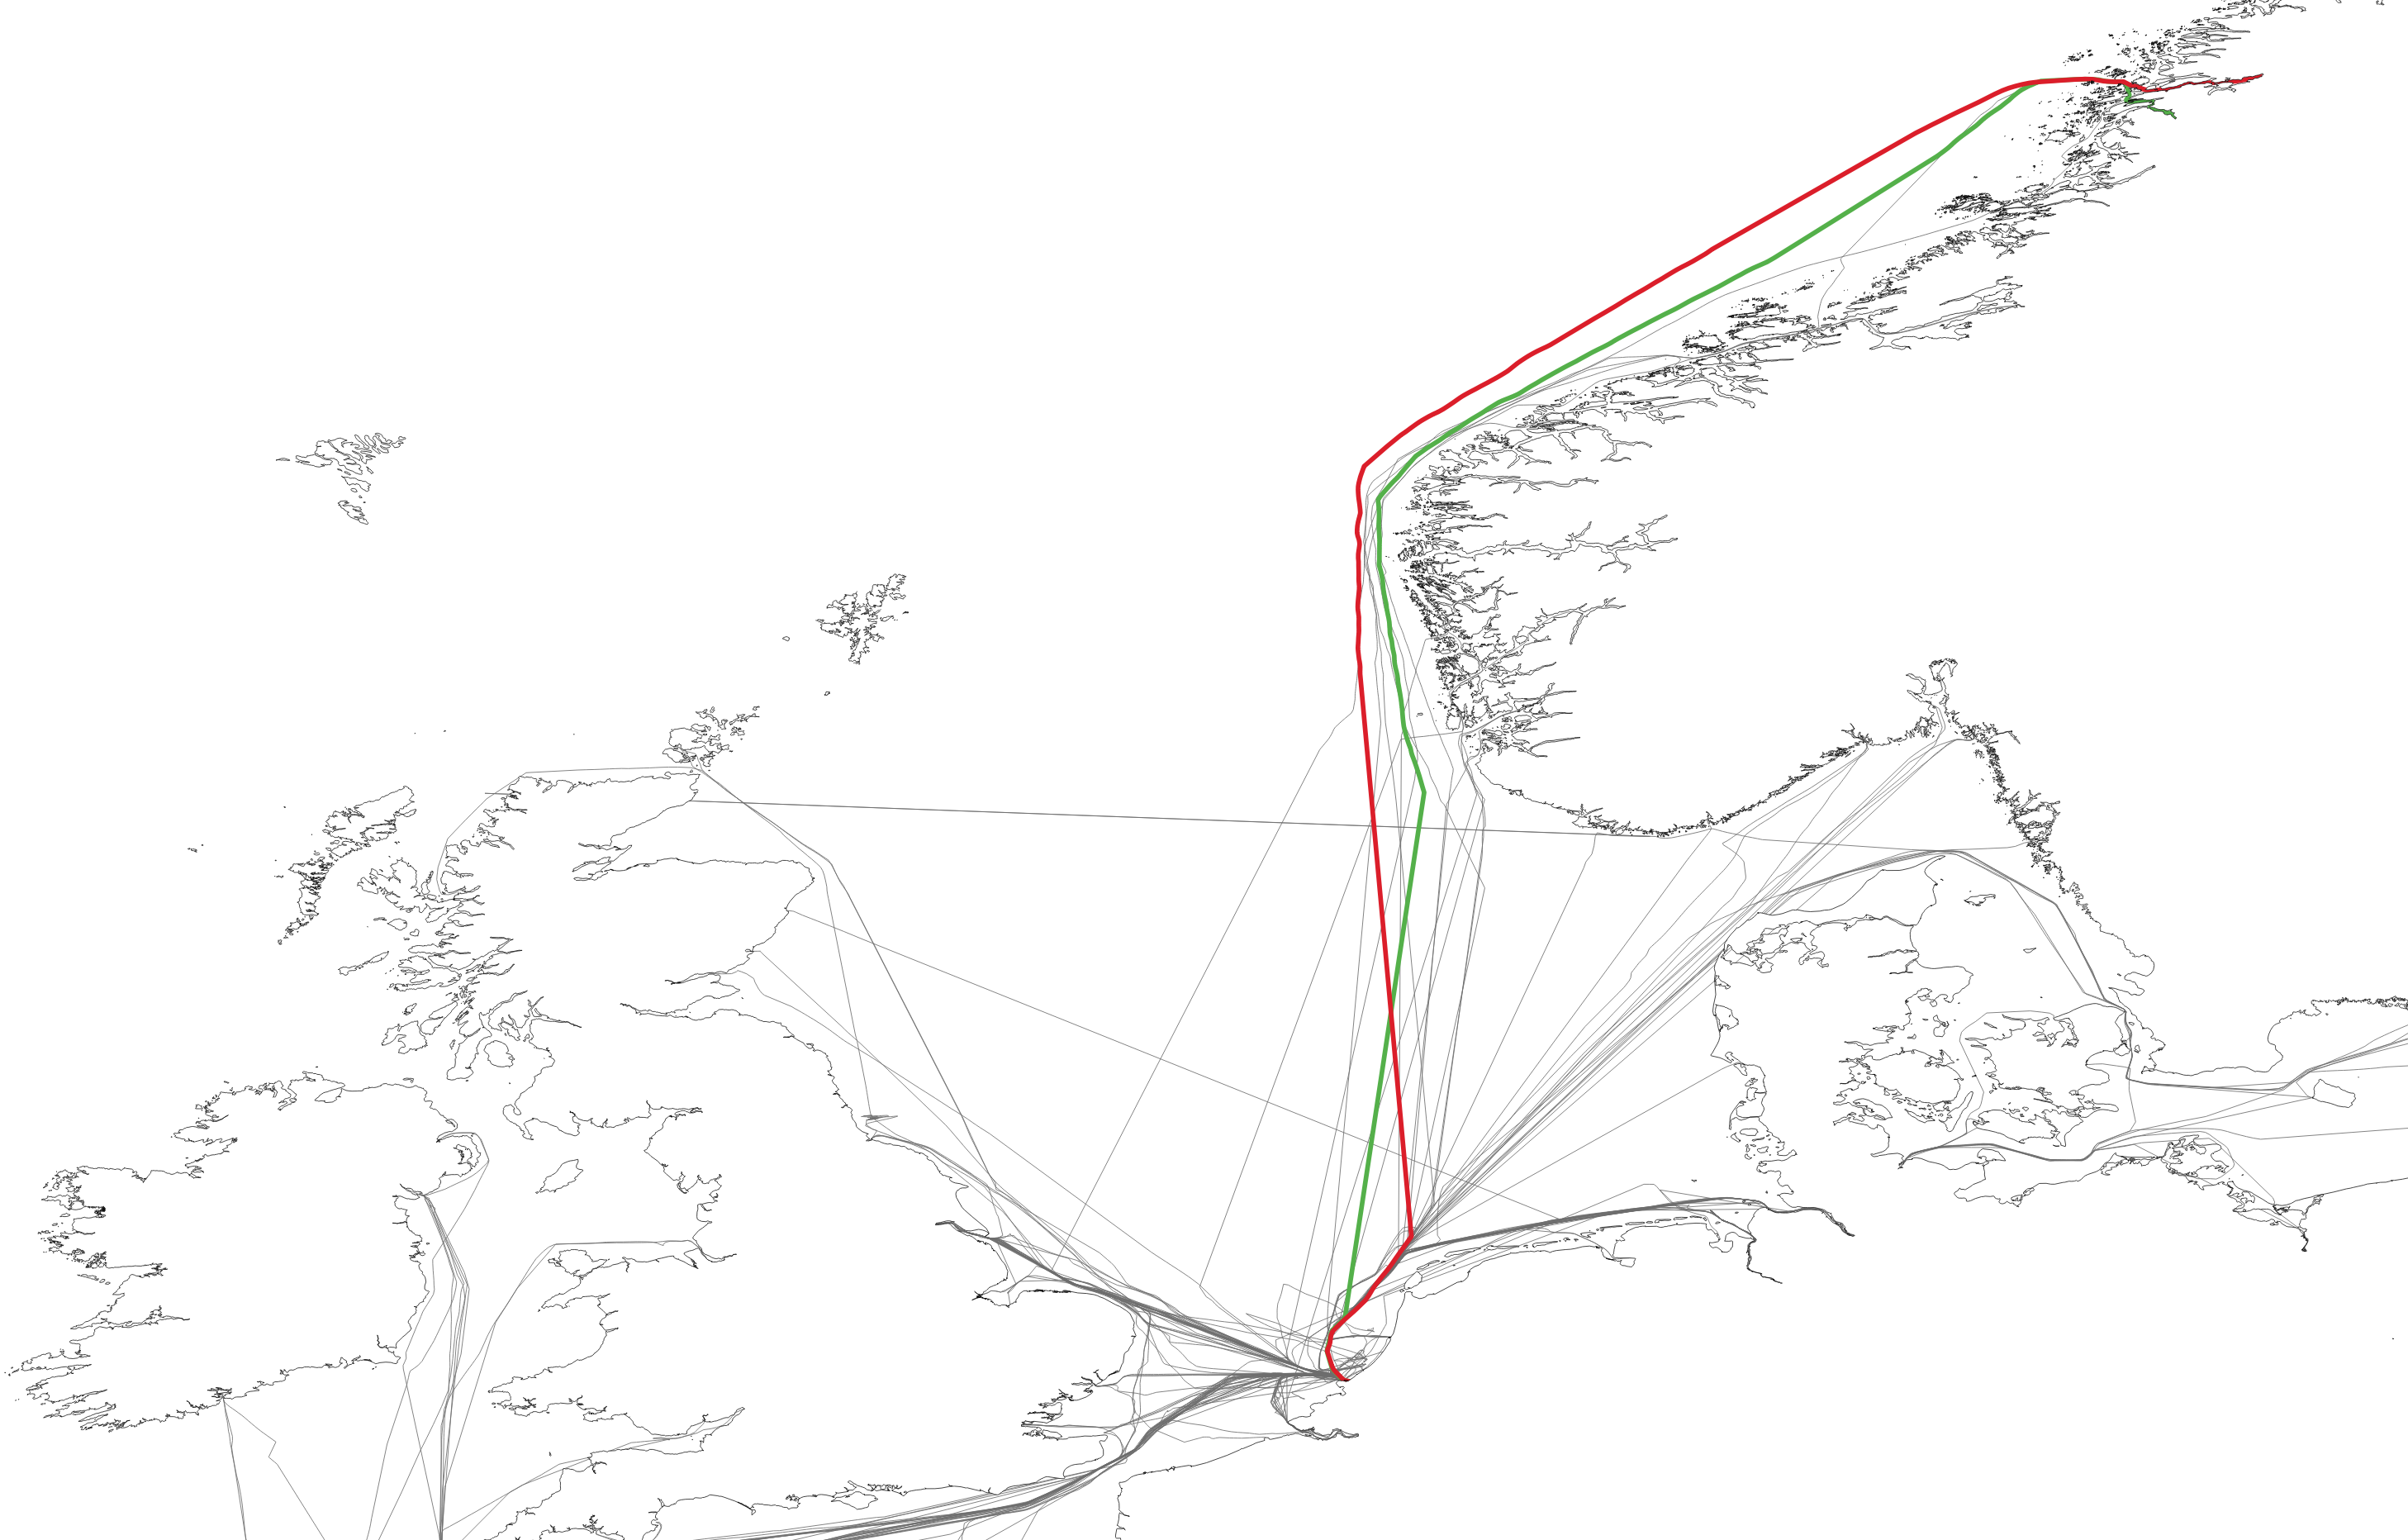
\includegraphics[width=1.0\textwidth]{figures/mstd}
    \caption{Example of \acrshort{mstd} for a given historical trajectory where the red line is the given trajectory and the green line is the most similar historical trajectory.}
    \label{fig:mstd}
\end{figure}


\subsection{Building ML data training set}

\begin{itemize}
    \item Batch calculating MSTD
    \item Different trajectory similarity approaches
    \item Adding more data attributes per voyage such as seasons, ballast/laden, etc\ldots
    \item Final result/structure
\end{itemize}

\subsection{Dataset imbalance}

\begin{itemize}
    \item Minority oversampling
    \item Majority undersampling
\end{itemize}

\subsection{Categorical label encoding}

\begin{itemize}
    \item Categorical values/labels must be encoded
    \item Label encoding vs one-hot encoding
\end{itemize}

\section{The final dataset summary}

The final process of creating the dataset used in the analysis can be summarized in the following steps:

\begin{itemize}
    \item Voyages are defined using time intervals provided by the vessels' \acrshort{ais} navigational status. They are constructed and stored in a voyage database table containing the full geographical trajectory, arrival and departure ports, and additional information for the traveling vessel.
    \item The voyage table's geographical trajectories are sampled, or simplified, based on a certain time interval to make trajecotory comparisons easier.
    \item Every sampled historical trajectory is split into multiple parts to emulate incomplete voyage, not yet arrived at a port. Furthermore, the \acrshort{mstd} is calculated for every one of these voyages. Trajectory similarity is defined using the \acrshort{sspd} algorithm, however, this data is interchangable with other similarity measurements.
    \item Finally, the \acrshort{mstd}, similarity value, trajectory length, departure and arrival ports, and vessel segmentation information is collected and stored as the \acrshort{ml} training data.
\end{itemize}

An overview of the processed described in this chapter thus far is shown in \cref{fig:dataset_overview} from the data provided by \acrfull{mo} to the final \acrshort{ml} training data.

\begin{figure}[htbp]  % order of priority: h here, t top, b bottom, p page
    \centering
    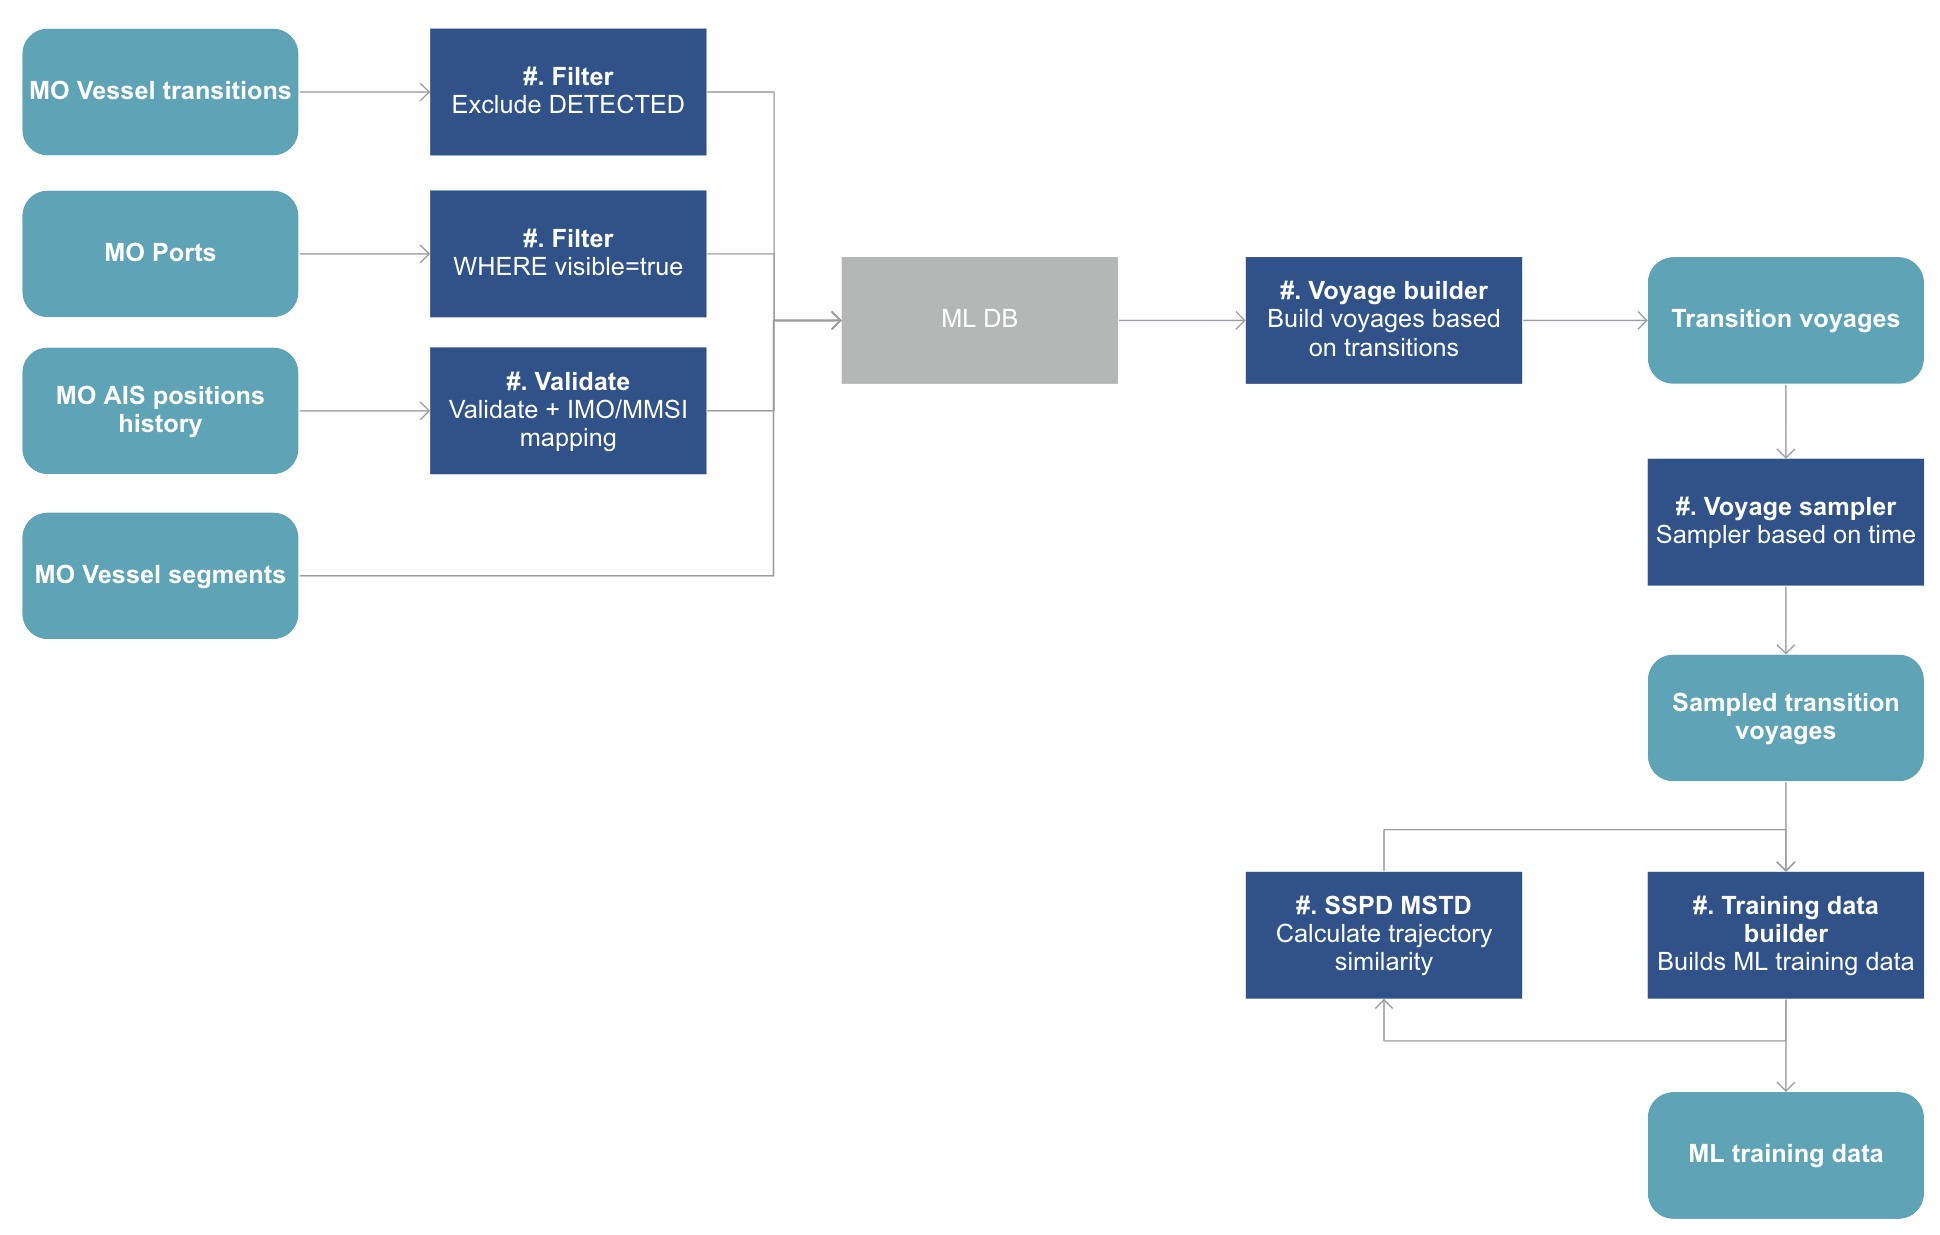
\includegraphics[width=1.0\textwidth]{figures/dataset_overview}
    \caption{Overview of the process used to construct the dataset used in further analysis and \acrshort{ml}.}
    \label{fig:dataset_overview}
\end{figure}


\section{ML-based training and destination prediction}

\subsection{Model selection}

\begin{itemize}
    \item Tree-based classifiers
    \item Multi-layered perceptrons classifiers
    \item Support-vector machines
    \item Multi-class classifiers vs OneVsRest binary classifiers
\end{itemize}

\subsection{Configuration and parameter optimization}

\subsection{Training}

\subsection{Evaluation process and metrics}

\begin{itemize}
    \item X-Folder-cross-validation
    \item Metrics: F1, precission, recall, AUC, vs accuracy
    \item Computing performance?
    \item How fast is it to compute the next destination of every vessel in the world
\end{itemize}

\section{Vessel destination prediction method summary}

Given the final trained model, the overall prediction process for a single traveling vessel can be conceptualized using the following steps:

\begin{itemize}
    \item The current trajectory of the traveling vessel is collected using \acrshort{ais} records ranging from the last transmitted \textit{``MOORED''} status to its current position along with the id (\gls{locode}) of the departure port where it was moored and the vessel's segmentation values.
    \item The vessel's trajectory is then sampled based on a predefined time interval, then compared to every historical outgoing trajectory from the same departure port from vessels of the same segment and sub-segment to establish the \acrfull{mstd}.
    \item The vessel's segment, sub-segment, departure port, trajectory length, \acrshort{mstd}, and the \acrshort{mstd} similarity value is then passed to a \acrshort{xgb} model that predicts the traveling vessel's arrival port.
\end{itemize}
